\chapter{État de l'art}\label{state_art_chap}

Tous les langages de programmation modernes définissent au moins une
représentation standard des chaînes de caractères, que ce soit
sous forme de tableau, de liste chaînée ou de corde.

Parmi les implémentations existantes, une majorité représente leurs chaînes
de caractères sous forme de tableau de caractères.
Malgré cette ressemblance, des différences de conception,
de codage et d'implémentation viennent changer la façon
d'interagir avec les chaînes de caractères d'un langage à
l'autre.
Ce chapitre a pour but de les introduire, et d'expliquer quels
sont les avantages et inconvénients de chaque implémentation.

Nous présentons d'abord les modèles de chaînes mutables et immutables,
puis nous comparons les avantages et inconvénients que chaque approche
offre.
Nous poursuivons sur une présentation des différentes structures de
données existantes à la rédaction de ce document: tableaux de caractères,
listes chaînées et cordes.
Nous terminons ce chapitre par les problématiques de codage, et plus
particulièrement d'Unicode.

\section{Mutable vs. Immutable}

Indépendamment de la structure, une chaîne de caractères peut être soit mutable,
soit immutable.
Une chaîne immutable est définie comme une chaîne dont le contenu ne peut pas
être modifié via des fonctions de manipulation.
Il est à noter cependant que la structure même des chaînes immutables peut être
mutable, par exemple pour des mécanismes d'amélioration de la performance comme
des systèmes de cache.

Parmi les langages de haut niveau populaires lors de la rédaction de ce document,
beaucoup préfèrent les chaînes de caractères immutables.
C'est le cas de Java \cite{java_spec}\footnote{Voir documentation à
\url{http://hg.openjdk.java.net/jdk8u/jdk8u/jdk/file/b95e325137b4/src/share/classes/java/lang/String.java},
\texttt{Strings are constant}.}, C\# \cite{csharp_spec}, Python \cite{pythonref}\footnote{Implémentation
disponible à \url{https://github.com/python/cpython/tree/c797daf69edc52385ba78447441e1a65c7cf5730/Objects/stringlib}.},
Scala \cite{scalaspec}, JavaScript \cite{ecmascript_spec}, etc.

À première vue, cette décision peut paraître limitante du fait qu'elle
empêche certaines opérations de façon efficace (concaténation,
modification, etc.). Cependant, elle assure la stabilité de la chaîne
de caractères tout au long de l'exécution du programme, et ce, peu importe le
nombre de modifications qu'elle subira, chaque modification entraînant une copie.
Cette propriété garantit un comportement sûr en programmation parallèle et concurrente.
En programmation séquentielle aussi, les structures immutables sont
généralement plus simples à manipuler du fait de l'absence d'effets de
bord à la modification.
Ces avantages induisent une meilleure stabilité et une probabilité de
comportement bogué plus faible.

L'immutabilité des chaînes de caractères permet également d'éviter
certaines opérations de copie en partageant des sous-parties de la
chaîne initiale.
Cela permet le support de certaines opérations
en temps constant au lieu de linéaire (substring, trim, etc.).

Les problèmes de concaténation et modification inefficaces ont été adressés
dans la plupart de langages ayant fait ce choix par l'introduction d'une
représentation mutable des chaînes de caractères: le \texttt{buffer}.

Cette structure permet d'effectuer des modifications
de la chaîne sans nécessiter de ré-allocation.
Cela a pour effet de combler les limites
apportées par l'immutabilité en permettant de modifier le contenu d'une
chaîne de façon efficace en général.
Des différences d'implémentation sont à noter en ce qui concerne les \texttt{buffers} en revanche.

Les langages utilisant des chaînes de caractères mutables ne subissent pas ces
désavan-tages et s'affranchissent du \texttt{buffer}.
C \cite{cspec}, C++ \cite{cppspec}, Fortran \cite{fortranspec} et d'autres langages
de bas-niveau en font partie.
Leur choix peut s'expliquer du fait de l'orientation performance et bas-niveau
de cette famille de langages.
Il est à noter cependant que le manque de métadonnées pour la longueur
de la chaîne dans certains de ces langages (voir~\ref{state_structs}) force les développeurs
à écrire leurs propres versions de chaînes mutables pour accélérer l'opération
de concaténation.

En plus de ces langages orientés performance, certains langages de plus haut-niveau utilisent
des chaînes mutables.
Ruby \cite{rubyref}\footnote{Implémentation disponible à
\url{https://github.com/ruby/ruby/blob/trunk/string.c}.} en est un exemple.
Une fonction définie sur les objets, \texttt{freeze}, permet de garantir la non-mutabilité
du receveur en provoquant une exception en cas de mutation.
Ruby utilise aussi des conventions de nommage pour discriminer les opérations altérantes
des opérations de copie: si le nom du service est suffixé par '!', il s'agit d'un service
mutatif, sinon, il produira une copie.

Le tableau~\ref{mutable_langs} récapitule les différents langages et leurs politiques vis-à-vis de
la mutabilité de leurs structures.

\begin{table}
	\caption{\label{mutable_langs}Langages et structures}
	\centering
	\begin{tabular}{lll}
		\hline
		Langage & Immutable & Mutable \\
		\hline
		Java & String & StringBuffer ou StringBuilder \\
		C\# & String & StringBuilder \\
		C & char* (lorsque chaînes litérales) & char* \\
		Ruby & frozen String & String \\
		Python & str & / \\
		Perl & Str & Buf \\
		Nit & String & Buffer\\
		Swift & string & / \\
		Go & string & / \\
		C++ & char* (lorsque chaînes litérales) & std::string \\
		\hline
	\end{tabular}
\end{table}

\section{Structures de données}\label{state_structs}

Il existe plusieurs structures pour représenter les chaînes de caractères dans les langages
de programmation.
Nous nous intéressons seulement ici aux structures destinées au stockage des chaînes
de caractères pour une utilisation générique.
La littérature existante dans ce domaine est très faible dans la mesure où les
programmeurs et implémenteurs de langages se contentent généralement de chaînes plates.
Des structures spécialisées et les algorithmes liés à ces structures sont, ou ont été
un sujet de recherche actif: tri \cite{bentley1997, hat_trie},
hachage \cite{pearson1990fast, mckenzie1990selecting},
recherche \cite{suffix_arrays, boyer1977fast}, etc.

Cette section les détaillera et exposera leurs avantages et inconvénients.
Nous commençons par le tableau de caractères dû à sa simplicité et sa popularité.
Nous présentons par la suite la liste chaînée, représentation favorite des langages
fonctionnels.
Puis nous terminons cette section par une structure souvent oubliée: la \texttt{corde}.

\subsection{Tableau de caractères}\label{state_flatstr_prez}

Nous commençons par la structure la plus ancienne et la plus populaire pour la
repré-sentation du texte: le tableau de caractères, tel qu'illustré dans la figure~\ref{flatexample}.
Du fait de la linéarité de la structure, nous allons ré-utiliser les termes de
Boehm \cite{Boehm95}, et qualifier cette représentation de «chaîne plate» dans le reste
de ce document.

Il existe deux représentations de cette structure:
\begin{enumerate}
	\item Les chaînes C, terminées par un caractère nul (illusté par \texttt{\textbackslash0} dans notre exemple).
	\item Les chaînes Pascal, représentées comme des structures contenant un premier champ de longueur, suivi du contenu de la chaîne.
\end{enumerate}

Du fait que dans les langages comme C, la chaîne ne possède pas d'information de longueur dans sa
structure, il a été décidé de terminer les chaînes de caractères par l'octet 0x00 et les fonctions
C travaillant sur des chaînes se servent de cette sémantique pour déterminer
la fin du traitement.
Cette sémantique est à l'origine de nombreuses failles de sécurité comme des dépassements
de tampon et leur prévention est laissée au programmeur, complexifiant le code.
Les chaînes Pascal évitent ce problème en incluant la longueur directement dans les données de la structure.
Cependant, ces dernières forcent la chaîne à se limiter à la taille de la donnée contenant
l'information de longueur et dépend donc de l'architecture cible pour le programme.

\begin{figure}
	\caption{Chaîne de caractères plate}
	\label{flatexample}
	\centering
	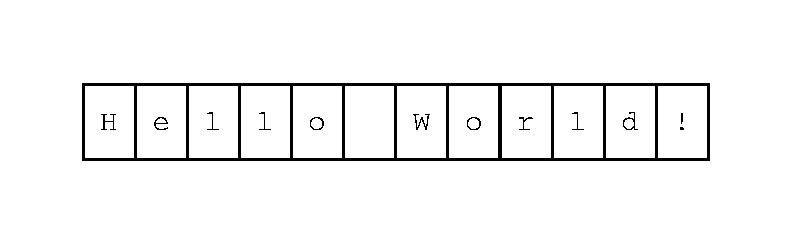
\includegraphics{figures/flat.pdf}
\end{figure}

Indépendamment de l'implémentation, qu'elle soit similaire à C, ou à Pascal, la structure possède
ses avantages et inconvénients.

Avantages:
\begin{enumerate}
	\item accès indexé constant à un codet;
	\item bonne performance en cache.
\end{enumerate}

Inconvénient:
\begin{enumerate}
	\item besoin d'espace contigu.
\end{enumerate}

Du fait de cet inconvénient, cette représentation des chaînes de caractères peut
dégénérer assez rapidement en terme d'espace et de coût.
En effet, lorsqu'une chaîne de caractères mutable est pleine, il faut réallouer
un espace plus grand et copier les anciennes données vers le nouvel espace.
Cette opération est peu coûteuse sur les chaînes de caractères de petite taille, les
coûts d'allocation et de copie étant négligeables dans ce cas.
En revanche cela peut dégénérer sur de grandes chaînes de caractères.

Ce problème des chaînes plates est encore aggravé avec l'immutabilité,
dans la mesure où la moindre opération de mutation entraîne une
réallocation complète de la chaîne.
L'impact de cette ré-allocation est généralement réduit dans les implémentations
de \texttt{buffer} par le biais de sur-allocations.
L'approche ici est de pré-allouer une quantité de mémoire supérieure à ce qui est
demandé pour amortir les coûts de l'allocation et de la copie sur un nombre suffisant de
concaténations.
La performance exposée ici est dans le cas général, suffisante pour les opérations
de concaténation multiples, les cas dégénératifs (insertion non-terminale d'une
chaîne) exposés par cette solutions étant rares, il est par conséquent peu fréquent
que les bibliothèques proposent une solution efficace et standard à ces problèmes.

\subsection{Liste chaînée}

Dans le monde fonctionnel, la représentation en tableau est bien souvent éclipsée
par la liste chaînée, représentée dans la figure~\ref{llistexample}.
Les langages hérités de Lisp utilisent cette structure.
C'est également le cas d'Haskell.

\begin{figure}
	\caption{Exemple de liste chaînée}
	\label{llistexample}
	\centering
	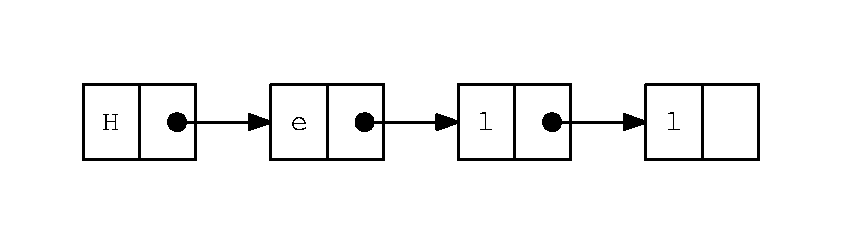
\includegraphics{figures/linked_list.pdf}
\end{figure}

Elle possède certains avantages par rapport à un tableau, notamment la capacité d'extension
en temps constant\footnote{Lorsque la mutabilité des structures est supportée, sinon l'opération
effectuée en temps linéaire.}.
Notons que si l'opération d'insertion s'effectue en temps constant, l'opération de
recherche du point d'accès se fait néanmoins en temps linéaire, à l'exception éventuellement
des extrêmités.
Il est également possible d'amortir l'opération en temps constant par le
biais d'un système de cache.

La représentation est néanmoins peu populaire dans les langages procéduraux et à objets, le
désavantage majeur de la solution est sa faible performance dans le cas de sous-chaînage,
ce dernier nécessitant la réallocation de chaque caractère afin de produire une nouvelle
chaîne.
L'itération, bien que théoriquement aussi performante qu'une approche par tableau, est mise à
mal par les caractéristiques des processeurs modernes de par son impossibilité à être
mise en cache efficacement.
La problématique de l'utilisation mémoire est aussi à prendre en compte.
En effet, chaque caractère est stocké dans un maillon; sa taille est donc la somme de
la taille du caractère et d'un un pointeur, au minimum.

\subsection{Corde}

Une autre alternative existe: la \texttt{corde} \cite{Boehm95}, illustrée dans la figure~\ref{ropeexample}.

\begin{figure}
	\caption{Exemple de corde}
	\label{ropeexample}
	\centering
	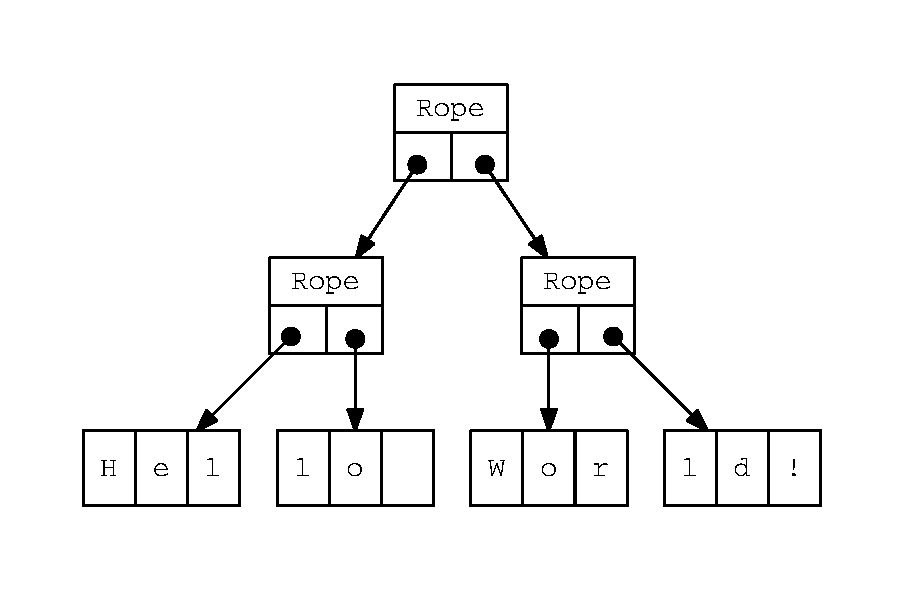
\includegraphics{figures/rope.pdf}
\end{figure}

Une corde est un arbre binaire accessible par index.
Chaque noeud de l'arbre est un noeud représentant une concaténation.
Les \texttt{feuilles} quant à elles sont des chaînes de caractères plates.

La structure propose de réduire la complexité d'opérations comme la concaténation à un
temps constant en remplacant l'allocation et la copie du contenu des chaînes par
la création d'un noeud de concaténation.
Cet avantage est néanmoins à nuancer du fait de la nécessité de ré-équilibrer la corde
périodiquement pour assurer les bonnes performances de la structure.
Elle permet également de réduire la complexité temporelle des opérations comme
l'insertion dans une chaîne à O(log(n)).
Cette opération s'effectue en trois étapes:

\begin{enumerate}
	\item le parcours jusqu'a la feuille à séparer (O(log(n)) si la corde est équilibrée);
	\item la séparation en deux parties à l'index d'insertion (complexité équivalente à deux substring + deux allocations de noeud de concaténation);
	\item la ré-écriture du parcours jusqu'a la racine (O(log(n))).
\end{enumerate}

Avantages:
\begin{enumerate}
	\item concaténation efficace en temps et en espace;
	\item potentiel de partage des feuilles (moins d'allocations).
\end{enumerate}

Inconvénients:
\begin{enumerate}
	\item accès en O(log(n)) aux feuilles de la chaîne;
	\item besoin de garder la structure équilibrée pour maintenir la complexité en O(log(n)).
\end{enumerate}

Malgré son introduction il y'a près de 20 ans, cette structure n'est
jamais devenue populaire, et a fini par tomber dans les limbes.
Cependant, il y'a eu des cas de re-découverte dans lesquels les cordes
étaient plus pertinentes à utiliser que des chaînes plates comme les éditeurs de
texte \cite{inria_rope}.

\subsection{Conclusion}

Parmi les langages modernes, peu proposent une alternative à la chaîne plate comme structure de
données pour les chaînes de caractères.
En dehors des langages à objets ou procéduraux, la liste chaînée est privilégiée dans les
langages fonctionnels, qui eux aussi évitent la corde.
Nit est donc un des rares langages à intégrer les cordes dans leur bibliothèque standard.
Julia~\cite{bezanson2012julia} propose également les cordes, cependant elle est dépréciée\footnote{
\url{https://github.com/JuliaLang/julia/blob/86cd5ea3c61426ebddd1d3809ffa869d6726fb30/base/deprecated.jl}}
pour des raisons de peformance, ceux-ci ne proposant pas de système de conversion, elle doit être
explicitement instanciée par les utilisateurs.
Ces derniers en abusant, les performances diminuaient, ce qui a mené à sa dépréciation.

\section{Codage}

Les chaînes de caractères en tant que telles sont des séquences de caractères.
Selon le codage utilisé, la définition de caractère peut varier.

À l'origine, il n'existait pas de standard pour la représentation des caractères.
Chaque système possédait sa variation d'une correspondance entre données binaires
et caractères.
À l'apparition des cartes perforées, les codages des caractères étaient propriétaires.
Chaque producteur de cartes possédait son propre codage, ce qui empêchait
l'interopérabilité entre différents fabricants.

Simultanément, en 1963, deux codages sont apparus et seront la base des deux grandes
familles de codages ayant façonné l'histoire de l'informatique: \textit{American Standard
Code for Information Interchange} (ASCII) \cite{ASA63} et \textit{Extended Binary Coded Decimal
Interchange Code} (EBCDIC) \cite{amdahl1964architecture}.
Le premier étant un effort de l'\textit{American Standards Association} (ASA), ancêtre de 
l'\textit{American National Standards Institute} (ANSI) et devenant un standard de facto au
départ, avant sa normalisation par ISO/IEC via l'ISO/IEC-646 \cite{ISO72}.
L'autre étant une extension du codage propriétaire d'IBM, \textit{Binary Coded Decimal},
déjà utilisé sur les cartes perforées du fabricant.

ISO/IEC-646 marque le début de la standardisation des codages de caractères en informatique.
Il définit une multitude de codages sur 7 bits pour les caractères de l'alphabet latin.
Il est suivi, dans les années 1980 des variantes de l'ISO/IEC-8859 ou ECMA-94 \cite{ECMA94} du côté européen.

Les limites de l'ASCII ou de l'ISO-8859 se sont vite fait ressentir dans les pays étrangers, si bien
qu'une multitude de codages ont commencé à appraître dans le monde entier; JIS X 208 \cite{JISX208}
pour le Japon, GOST 10859 \cite{GOST64} pour l'URSS, remplacé plus tard par KOI-8 \cite{KOI8} et ses
dérivées, GB2312 \cite{GB2312} pour la Chine, les variantes de Big5 \cite{big5cite} pour Taiwan,
Hong-Kong et Macau, etc.

La multitude de codages rendait l'échange d'information entre les pays difficile, voire dans certains cas
à l'intérieur d'un même pays, ce qui motiva la création d'Unicode \cite{Unicode91}.
En conjonction avec l'ISO/IEC, le consortium Unicode et IEEE partici-pèrent à l'élaboration
d'\textit{Universal Character Set} (UCS) \cite{UCS1993}.

\subsection{UCS-2}

Quand les travaux sur Unicode ont commencé, en 1988, le standard à venir ne concernait
qu'un codage et une table de caractères; les deux étaient confondus \cite{Unicode88}.
L'espace prévu par Unicode pour décrire les caractères supportés était de 16 bits (65536 valeurs).
Chaque valeur définie dans le standard est appelée selon Unicode un \texttt{point de code}.
Pour coder cette information, UCS-2 (alors appelé Unicode) est décrit dans la première version du
standard \cite{Unicode91}.

Il s'agit d'un codage à longueur fixe, à l'instar de ISO-646 ou ISO-8859, chaque valeur possède
un caractère associé.
Du fait de ses codets de 16 bits, UCS-2 est vulnérable aux problèmes de boutisme, contrairement
aux codages utilisant l'octet comme codet.
Pour palier ce problème dans les fichiers, Unicode préconise l'utilisation d'un
BOM\footnote{Byte Order Mark, point de code 0xFEFF déterminant le boutisme d'un bloc de texte Unicode.}
dans les fichiers Unicode.
Si le fichier est codé en UTF-16, les deux premiers octets seront soit \texttt{0xFFFE} dans le cas de
petit-boutisme ou \texttt{0xFEFF} dans le cas de gros-boutisme.
À la publication d'ISO-10646 dans sa première version \cite{UCS1993}, il est l'un des deux codages couverts
par la norme, l'autre étant UCS-4.

\subsection{UCS-4}

UCS-4 est similaire à UCS-2 dans le sens où il propose un codage de longueur fixe.
La différence est que UCS-4 propose des codets de 32 bits au lieu de 16 bits.
La raison à cela est un conflit d'opinion entre le consortium Unicode et
le sous-groupe d'ISO/IEC responsable de la normalisation d'UCS.
Le Consortium Unicode était convaincu que 16 bits suffiraient pour coder l'intégralité
des caractères du monde entier, là où ISO/IEC proposait de normaliser un espace de
données de 32 bits coupé en plans de 65536 valeurs.
Pour les mêmes raisons qu'UCS-2, cette représentation est vulnérable aux problèmes de
boutisme.

Lors de la fusion des deux normes, les deux codages ont été ajoutés aux documents.
Unicode ne spécifiait que les 65536 premières valeurs et ISO/IEC supportait l'ajout
ultérieur de nouvelles valeurs dans l'espace disponible.

\subsection{UTF-8}

UTF-8 est un des codages définis par Unicode et ISO/IEC-10646.
La première version a été produite par Rob Pike et Ken Thompson dès
1992 et implémentée dans le système d'exploitation de recherche Plan9 \cite{Plan9}.

UTF-8 a été créé pour deux raisons principales; la première étant la rétro-compatibilité avec
ASCII et les chaînes de caractères C, terminées par un octet nul (0x00).
La deuxième raison est que les concepteurs d'UTF-8, conscients du différend de point
de vue entre Unicode et ISO/IEC, ne voulaient pas se borner aux 16 bits définis par
Unicode et étaient mécontents d'UCS-4 à cause de la perte d'espace occasionnée par les codets de 32 bits.
UTF-8 est donc un codage à longueur variable ayant pour codet l'octet.
Il est capable de coder l'intégralité des points de code supportés par ISO/IEC 10646.

Chaque point de code est codé sur une séquence de 1 à 6 octets.
Le premier octet de la séquence détermine la longueur de la séquence, par la suite,
chaque octet de la séquence doit respecter le motif '10'.
Le tableau~\ref{utf8_sequences} montre l'organisation des séquences UTF-8.

\begin{table}
	\caption{\label{utf8_sequences}Organisation des séquences UTF-8}
	\centering
	\begin{tabular}{llllll}
		\hline
		Point de code & Glyphe & Octet 1 & Octet 2 & Octet 3 & Octet 4\\
		\hline
		0x41 & A & 0x41 & & & \\
		0xC9 & É & 0xC3 & 0x89 & & \\
		0x3042 & {\fontspec{WenQuanYi Micro Hei}あ} & 0xE3 & 0x81 & 0x82 & \\
		0x1F60A & {\fontspec{DejaVu Sans}😊} & 0xF0 & 0x9F & 0x98 & 0x8A \\
		\hline
	\end{tabular}
\end{table}

\subsection{UTF-16}

À la version 2.0 d'Unicode, le nombre total de caractères définis a dépassé les 65536 prévus
à la base par Unicode.
Pour palier ce problème, le consortium Unicode a fait évoluer UCS-2 en UTF-16.

Le codage fonctionne par un systèmes de paires complémentaires et est capable de coder un total
de 1 114 111 caractères.
À la date de rédaction de ce mémoire, 120 737 points de code sont assignés \cite{Unicode8}.
De ce fait, le standard est limité depuis à ce nombre de points de code.
UTF-8 n'ayant plus besoin de supporter 2 milliards de points de code, sa spécification est simplifiée
et le nombre maximal de codets est limité à 4.
Des points de codes compris entre 0xD800 et 0xDFFF sont réservés pour coder les paires complémentaires
et ne sont valides qu'en UTF-16.

Le tableau~\ref{unicode_sequences} montre les différentes représentations possibles du caractère {\fontspec{DejaVu Sans}😊} 
en fonction des différents codages Unicode.

\begin{table}
	\caption{\label{unicode_sequences}Représentation du caractère {\fontspec{DejaVu Sans}😊} dans les codages Unicode}
	\centering
	\begin{tabular}{lllll}
		\hline
		Codage & Octet 1 & Octet 2 & Octet 3 & Octet 4\\
		\hline
		UTF-8 & 0xF0 & 0x9F & 0x98 & 0x8A \\
		UTF-16 BE & 0xD8 & 0x3D & 0xDE & 0x0A \\
		UTF-16 LE & 0x3D & 0xDE & 0x0A & 0xDE \\
		UTF-32 BE & 0x00 & 0x01 & 0xF6 & 0x0A \\
		UTF-32 LE & 0x0A & 0xF6 & 0x01 & 0x00 \\
		\hline
	\end{tabular}
\end{table}

\subsection{Support d'Unicode dans les langages de programmation}

Parmi les langages modernes, presque tous possédant des sémantiques liées à Unicode dans leur
gestion des chaînes de caractères.

Le niveau de support d'Unicode varie selon les langages, certains supportent les
opéra-tions de base de façon correcte vis-à-vis du standard.
D'autres supportent les extensions liées aux locales (ce qui est nécessaire pour
le tri par exemple).

Au niveau des codages par exemple, Java et C\# utilisent UTF-16 en interne,
les opérations de modification sont fonctionnelles avec des sémantiques
d'Unicode et offrent également des extensions de locales.

Python, avant sa version 3, offrait deux types de chaînes de caractères.
\texttt{str}, qui est composé de octets arbitraires, et \texttt{unicode}, composé
de codets UTF-16 \cite{PEP100}, ou de codets UTF-32 si l'interpréteur est compilé
pour les utiliser en interne.
Plus tard, une extension des caractères pousse le codage
des chaînes de caractères en UTF-32, si le programmeur le demande
explicitement.
En Python 3, le PEP 393 \cite{PEP393} change l'implémentation interne en codets ISO8859-1,
UTF-16 ou UTF-32 dépendamment du plus grand point de code de la chaîne.

Ruby ne définit pas de codage par défaut pour ses chaînes de caractères,
chacune d'elles possède son propre codage et les opérations qui les
manipulent sont différentes en fonction du codage de la chaîne.
Les deux raisons principales de cette approche sont:
\begin{enumerate}
	\item la réduction du nombre d'opérations de codage/décodage à la lecture ou l'écriture vers un média;
	\item une protection contre les problèmes à long-terme du choix d'un codage unique (dépréciation, évolution
de la norme, etc.).
\end{enumerate}

\subsection{Évolution des opérations avec Unicode}\label{unicode_troubles}

Avant l'arrivée d'Unicode, les opérations sur des chaînes de caractères étaient efficaces du fait
de la simplicité des normes et du codage sous-jacent.
Les comparaisons se basaient sur la valeur du codet, les manipulations pour changer la casse
des caractères se résumaient à des opérations arithmétiques ou des accès à une table.
Unicode vient bouleverser cette sémantique et complexifier l'ensemble des manipulations.

Prenons l'exemple de l'équivalence de chaînes de caractères; l'apparition de caractères combinants
vient complexifier l'opération dans la mesure où les combinaisons de points de code doivent
être résolues avant d'effectuer une comparaison entre deux chaînes (voir tableau~\ref{combining_example}).
Il existe également le problème de caractères isomorphes; des
glyphes\footnote{Représentation graphique d'un signe typographique.} représentant des caractères différents
sont équivalents ou tout du moins très similaires (exemple: le signe d'Angström Å et le A-Ring utilisé
dans les alphabets nordiques Å).
L'ensemble de ces cas doivent être pris en compte pour assurer une comparaison respectant le standard
Unicode.

\begin{table}
	\caption{\label{combining_example}Exemple de caractères combinants à glyphe équivalent}
	\centering
	\begin{tabular}{lll}
		\hline
		Glyphe & Point de code & Code Combinant \\
		\hline
		Å & U+00C5 &   \\
		Å & U+0041 & U+030A \\
		Å & U+212B &  \\
		\hline
	\end{tabular}
\end{table}

Il existe également une deuxième façon spécifiée de comparer deux chaînes: la compa-tibilité.
Il s'agit de permettre la prise en compte de versions sémantiquement égales mais graphi-quement différentes
d'un même caractère.
Sous cette forme de comparaison, les chaînes \og H2O \fg{} et \og H$_{2}$O \fg{} doivent être considérées
comme égales.

Si l'égalité canonique est prévisible et fiable, l'ordonnancement de caractères est autre-ment plus complexe
car dépendant de la locale, les lettres doivent être ordonnées différemment dans certains contextes.
Par exemple: \og ll \fg{} va être considéré comme deux lettres dans les pays d'europe, sauf en espagne où
\og ll \fg{} est
une ligature\footnote{Fusion de deux graphèmes d’une écriture pour n’en former qu’un seul nouveau.} considérée
comme une lettre indépendante, qui possède sa rubrique dans un dictionnaire ou un bottin téléphonique,
située entre le \og l \fg{} et \og m \fg{}.
Il existe également des cultures où il n'existe pas d'ordre officiel de comparaision (ex: Japon) et d'autres
où plusieurs ordres sont disponibles (ex: Allemagne).

Ces problèmes de sémantique amènent des problèmes de recherche de motifs: veut-on se baser sur
l'équivalence canonique ou sur de la compatibilité lors de la recherche? À quel point veut-on sacrifier de
la performance pour de la simplicité d'utilisation?

Des modifications comme \texttt{trim}\footnote{Suppression des caractères d'espacement au début et à la fin d'une chaine de caractères.}
deviennent également complexes dans la mesure où les espaces ne sont
plus confinés à un espace restreint comme ASCII ou ISO-8859 l'avaient défini, mais à toute la table
Unicode.
De plus, certains caractères sont reconnus comme des caractères d'espacement, mais n'en ont pas
nécéssairement l'air: U+1680 par exemple, est un caractère d'espacement en alphabet Ogham, un alphabet runique
irlandais, dont le glyphe ressemble à un \texttt{-}.

Les opérations de modifications de caractères sont elles-aussi dépendantes de la locale.
Par exemple le caractère \og i \fg{} va se transformer en \og I \fg{} pour la majorité des utilisateurs,
sauf en locale Turque, ou il sera représenté par le caractère \og İ \fg{}.
Par ailleurs, les opérations de modification de casse sont non symétriques.
En allemand, le caractère \og ß \fg{} se transforme en \og SS \fg{} une fois en majuscule, qui eux, se transforment
en \og ss \fg{} une fois en minuscule.
Cette sémantique pose également un problème pour les API retournant un caractère lors de
l'opération dans la mesure ou un caractère unique peut se transformer en une chaîne de
caractères.

\subsection{Définition: caractère}

Dans la mesure où une chaîne de caractères est une suite de caractères,
un point sur lequel tous les langages pourraient à priori sembler
d'accord est la notion même de caractère.

En réalité, il n'existe pas de consensus concernant le caractère.
Il peut être une entité complètement différente d'un langage
à l'autre.
Parfois pour des raisons historiques (Java et ses codets UTF-16), parfois
de vision (Go avec UTF-8 ou Swift avec ses Extended Grapheme Clusters), voire dans
certains cas la notion est inexistante (Ruby, Python, etc.).

C et C++ considèrent des chaînes de caractères comme des
tableaux d'octets terminés par un octet 0x00.
Avec l'arrivée d'Unicode, un type \texttt{wchar\char`_t} a été ajouté au standard
pour supporter les codages comme UTF-16 ou UTF-32.
Cet ajout n'est cependant pas exempt de défaut et certains projets comme
GNU libunistring\footnote{The \texttt{wchar\char`_t} mess - \url{https://www.gnu.org/software/libunistring/manual/html_node/The-wchar_005ft-mess.html}.}
critiquent avec véhémence le type de données du fait de son manque de standardisation,
de sa faible utilité dans les implémentations limitant sa taille à 16 bits, ainsi que
de la fragilité des API associées.

Des langages plus haut-niveau comme Java \cite{java_spec} définissent leurs caractères comme
des codets UTF-16.
Ils ont une taille fixe de 16 bits et la gestion des paires d'extension est laissée
au programmeur.
C\# \cite{csharp_spec} et Javascript \cite{ecmascript_spec} le définissent de façon similaire.

Go \cite{goref} définit un concept analogue à un point de code nommé
Rune, à l'instar des Runes défninies par Plan9 \cite{Plan9}.
Leurs chaînes de caractères sont en fait des tableaux d'octets et ils
possèdent des opérations pour les traiter comme de l'UTF-8, 16 ou 32, le codage des chaînes
étant UTF-8 par défaut.

Swift \cite{swiftref} est un des rares langages statiquement typés et compilés à définir un
caractère comme une structure non primitive.
En Swift, un caractère est défini comme un ensemble étendu de graphèmes \cite{Unicode8}.
Il s'agit d'une séquence d'un ou plusieurs points de code, qui
combinés, produisent un caractère lisible par un être humain.

D'autres langages comme Ruby ou Python sont complètement dépourvus de la notion de
caractère, et un accès à une chaîne de caractères renvoie systématiquement
une sous-chaîne.
Perl, dans sa version 6, définit plusieurs niveaux d'accès aux éléments d'une chaîne:
octets, points de code, graphèmes.

\subsection{Conclusion}

La notion de codage est variable selon les langages (voir tableau~\ref{coding_recap}).
Certains définissent un codage par défaut, d'autres en supportent explicitement
plusieurs, voire certains ne font pas de distinction entre objet binaire et chaîne
de caractères.
De cette notion découle directement la notion de caractère, elle aussi ambigüe.

\begin{table}
	\caption{\label{coding_recap}Codage, selon les langages}
	\centering
	\begin{tabular}{llllll}
		\hline
		& Aucun & Variable & UTF-8 & UTF-16 & UTF-32 \\
		\hline
		Java & Non & Non & Non & Oui & Non \\
		C\# & Non & Non & Non & Oui & Non \\
		C & Oui & Non & Non & Non & Non \\
		Ruby & Non & Oui & Oui (défaut) & Oui & Oui \\
		Python & Non & Oui & Non & Oui (UCS-2) & Oui \\
		Perl & Non & Oui & Oui (défaut) & Oui & Oui \\
		Nit & Non & Non & Oui & Non & Non \\
		Swift & Non & Non & Non & Oui & Non \\
		Go & Non & Oui & Oui (défaut) & Oui & Oui \\
		\hline
	\end{tabular}
\end{table}

\section{Opérations primitives}

Nous identifions trois opérations primitives des chaînes de caractères dans cette étude.
Ces trois opérations serviront à implémenter l'ensemble des opérations sur des chaînes
de caractères et détermineront la complexité globale sur ces dernières.

\subsection{Concaténation}

Le processus de concaténation est la création d'une nouvelle chaîne de caractères à partir
de deux morceaux, eux-mêmes des chaînes de caractères indépendantes.
L'opération est effectuée de plusieurs façons dans les langages actuels.

Java et C\# par exemple travaillent avec des chaînes de caractères plates, l'utilisation de
l'opérateur de concaténation provoque l'allocation d'un nouvel espace pour le
contenu des deux chaînes et la copie avant de stocker cet espace dans un nouvel objet.
Il est à noter que dans ces deux langages, le cas où plusieurs concaténations sont syntaxiquement effectuées
à la suite est optimisé et les concaténations individuelles sont remplacées par un \texttt{buffer}
et des ajouts mutables.

Ruby possède plusieurs façons de concaténer des chaînes, l'opérateur + ou l'opérateur \textless\textless.
La différence entre les deux est que \textless\textless est mutatif (et donc non-sûr
dans la mesure où un objet peut être \texttt{frozen}\footnote{Rendu immutable par la fonction freeze du langage.})
là où + crée une copie.
De par son caractère mutatif en revanche, \textless\textless  est plus efficace.

Des langages comme Python, ne possèdant pas de chaînes mutables,
conseillent de passer par des tableaux de chaînes dans le
cas de concaténations multiples, puis de joindre l'ensemble.
Il existe également un opérateur + pour la concaténation simple.

\subsection{Accès indexé}

Une autre opération fréquente sur des chaînes de caractères est l'accès à un caractère
de la chaîne.
Dépendamment de la définition de caractère, l'opération change de sens.

La définition de Java selon laquelle un caractère est un codet UTF-16 lui permet d'offrir
au programmeur une complexité temporelle en O(1) pour l'accès à un caractère, peu importe
sa position dans la chaîne.
Le problème de cette approche est que selon Unicode, un point de code est potentiellement
codé sur 32 bits, laissant au programmeur le soin de gérer les paires complémentaires.
Il s'agit d'un problème récurrent dans les implémentations des chaînes utilisant UTF-16
(C\# et Python 2.x souffrent du problème par exemple),
qui peut sembler fonctionnel tant que le texte contient uniquement des caractères du 
BMP\footnote{Basic Multilingual Plane, les 65535 premiers caractères de la norme Unicode,
représentant les langues vivantes actuelles.}; le cas le plus fréquent.
Cependant, lorsque le texte contient des caractères en dehors de ce plan, un accès indexé
ne renverra qu'une partie de ce caractère, provoquant des comportements bogués.

Des langages comme Go fournissent une interface de récupération de Runes respectant
le standard établi par Unicode.
En UTF-8 ou UTF-16, les codages étant de longueur variable, l'accès à un caractère
est donc en complexité O(n).
UTF-32 étant également supporté par le langage et de par son statut de codage à
longueur fixe, il offre un accès en temps constant.

Des langages comme Swift, traitant les caractères comme des graphèmes, sont
obligés de gérer les possibilités de points de code combinants\footnote{Façon de gérer les caractères avec diacritiques par un système de combinaison.}
suivant un point de code quelconque.
Une première opération de récupération d'un caractère est effectuée en un premier temps, de complexité
temporelle linéaire.
S'en suit une phase de lookahead pour déterminer la présence de caractères combinants.
Cette opération est potentiellement dégénérative, Unicode ne limitant pas le nombre de
caractères combinants après un caractère de base.

\subsection{Sous-chaînage}

La dernière opération fondamentale des chaînes de caractères est la production de
sous-chaînes.
Lorsque l'on travaille avec des chaînes de caractères, il est souvent nécessaire
de travailler sur des sous-parties d'une plus grande chaîne.
La façon simple de procéder est d'en extraire une sous-chaîne indépendante sur
laquelle effectuer un traitement ultérieur.

Il existe deux façons principales de produire des sous-chaînes: par copie ou par référence.
La copie est utilisée en C\# par exemple; à chaque appel à \texttt{substring}
un nouvel espace est alloué et le contenu de la chaîne est copié, occasionnant une
complexité temporelle et spatiale de O(n).
L'avantage de la manoeuvre est que la chaîne de base n'est plus référencée et peut être
désallouée de façon sûre.
Le principal désavantage vient des manoeuvres de réallocation et copie qui dégénèrent
sur de grandes chaînes.

Java est également de ces langages à allouer de nouvelles chaînes à chaque appel à
\texttt{substring}.
Cependant, ce n'est le comportement par défaut que depuis la version 7 update 6.
Avant cela, les données de la chaîne étaient partagées entre plusieurs instances,
le début de la chaîne était stocké dans la structure elle-même sous la forme d'un
décalage et d'une longueur pré-définie.
La raison de ce changement est au niveau de l'utilisation de la mémoire, les sous-chaînes
empêchant le ramassage de la chaîne parente, si cette dernière est large, elle peut
occasionner des problèmes de capacité mémoire.
Un autre point invoqué est la non-applicabilité de la complexité O(1) sur une chaîne
de petite taille; essentiellement, une allocation et une copie pour un petit espace
de données est négligeable par rapport au
maintien des indices et aux coûts additionnels des opérations
dans le cas d'une chaîne partagée.

\section{Conclusion}

Ce chapitre présente les différents points de variabilité des chaînes de caractères dans les
langages de programmation.
Qu'il s'agisse de différences structurelles, de codage ou de mutabilité; chaque langage possède
une idée qui lui est propre de la chaîne de caractères.
Ces choix possèdent tous des avantages et des inconvénients, et il n'existe pas, ni n'existera
un jour, de chaîne de caractères parfaite, dépourvue d'inconvénients.
En revanche, il est possible de limiter les inconvénients de chaque approche, tout en
gardant les avantages de chaque représentation.
Le prochain chapitre présente la solution que nous avons implémentée en Nit, et qui représente
selon nous un bon compromis entre tous les points soulevés ici.
